\begin{pregunta}
\puntaje{5}
\begin{cuerpo}
La implementaci\'on del m\'etodo de Euler del siguiente rutero de Matlab 
\begin{lstlisting}
f=@(t,v) 0.3-0.1/exp(-0.01*t)
t=0:0.1:500;
v(1)=8;
for i=1:length(t)-1
    v(i+1)=f(t(i),v(i))*0.001+v(i);
end
plot(t,v)
\end{lstlisting}
genera la gr\'afica de la soluci\'on num\'erica del P.V.I. 
\begin{center}
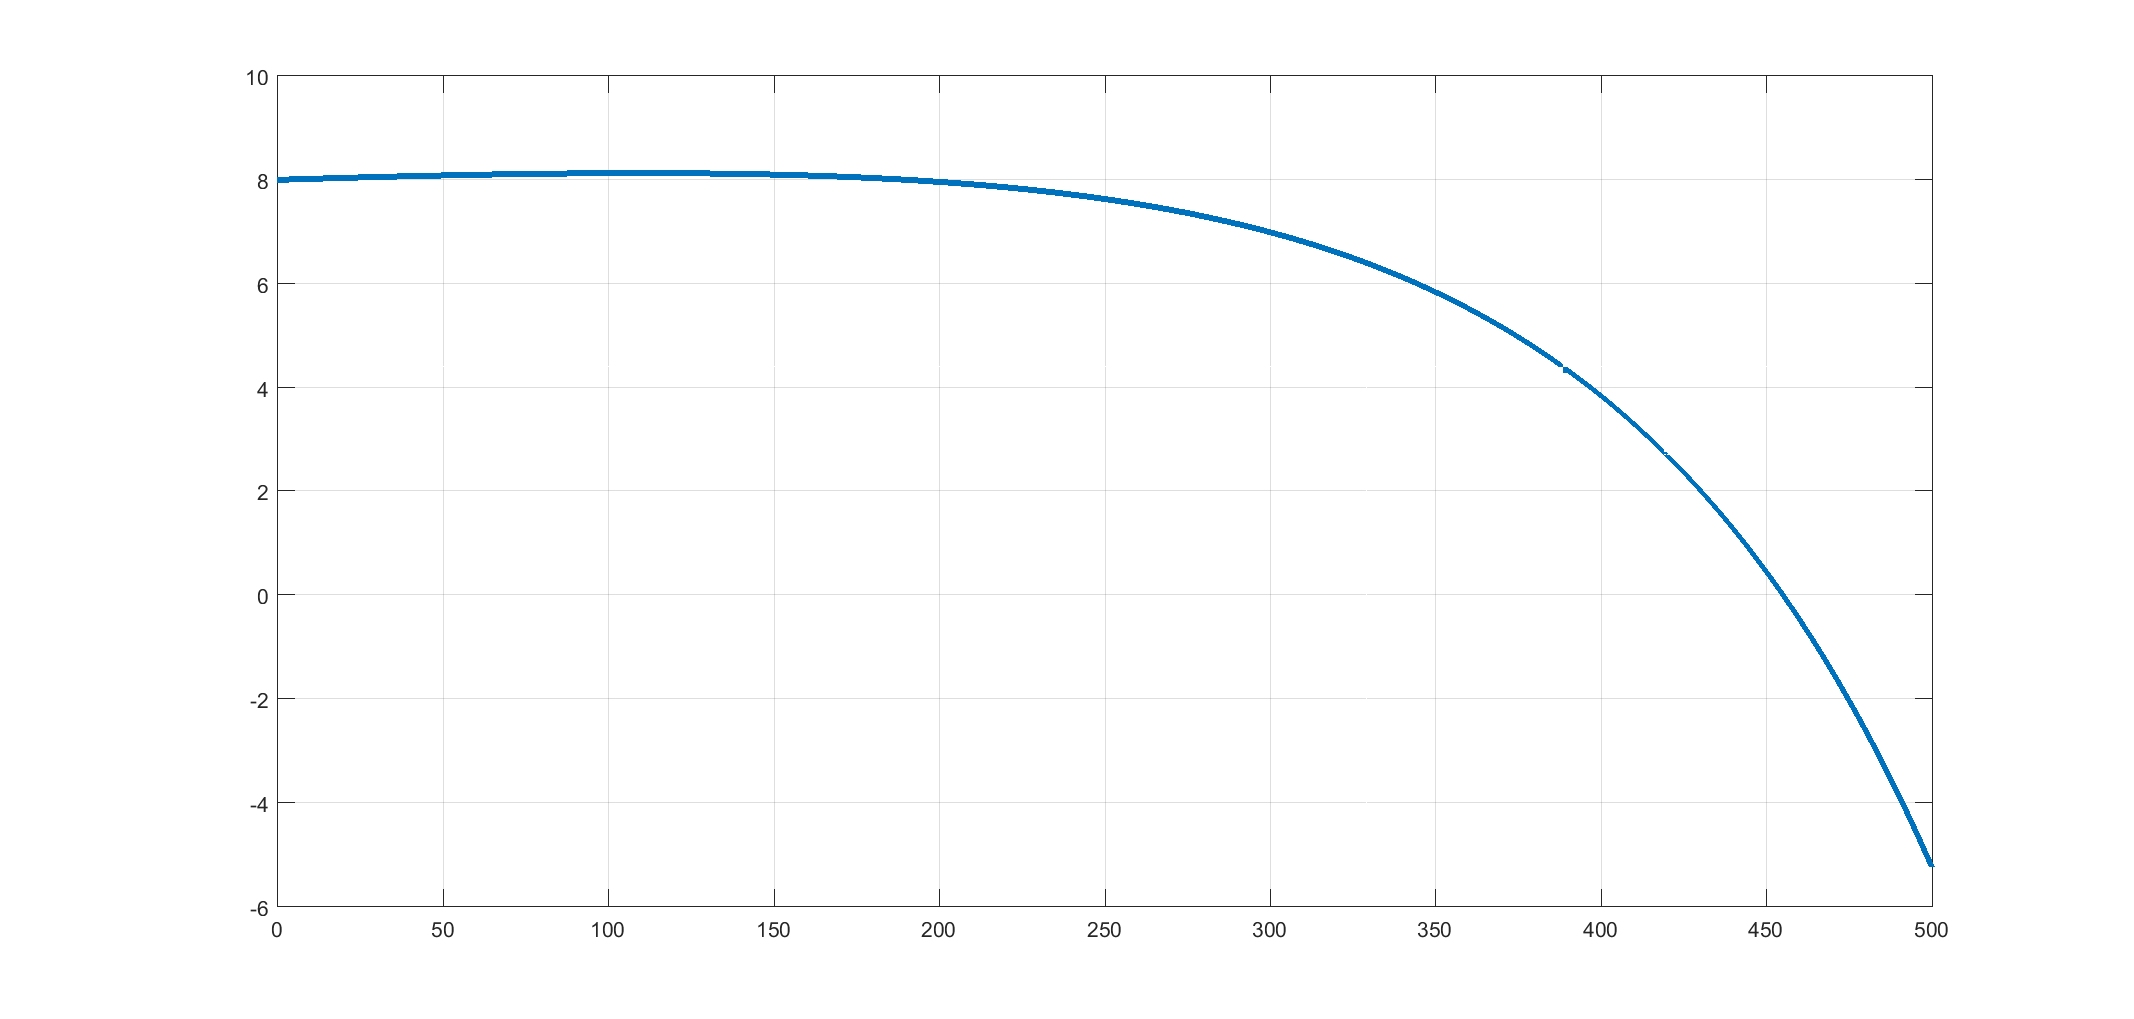
\includegraphics[width=\textwidth]{./img/p17.jpg}
\end{center}
para encontrar el valor de la variable independiente \texttt{t} donde la soluci\'on num\'erica cambia de signo, podemos ejecutar
\end{cuerpo}

\begin{multicols}{2}
\begin{alternativas}
{\texttt{t(min(find(v>0)))}}
{\texttt{v(min(find(v<0)))}}
{\texttt{t(max(find(v<0)))}}
{\texttt{t(min(find(v>0)))}}
\end{alternativas}
\end{multicols}
\justificacion{0cm}
\end{pregunta}